\documentclass[12pt,a4paper]{article}
\usepackage[utf8]{inputenc}
\usepackage{amsmath}
\usepackage{textcomp}

\usepackage{geometry}
\geometry{a4paper,left=25mm,right=25mm, top=2cm, bottom=2cm} 

\usepackage{verbatim}

 \usepackage{mathptmx}
 \usepackage[scaled=.90]{helvet}
 \usepackage{courier}

\usepackage[utf8]{inputenc}

\usepackage{listings}
\usepackage{color}

\usepackage{graphicx}
 
\definecolor{dkgreen}{rgb}{0,0.6,0}
\definecolor{gray}{rgb}{0.5,0.5,0.5}
\definecolor{mauve}{rgb}{0.58,0,0.82}

\pagestyle{empty}
\lstset{numbers=left,language=C++}
\lstset{showstringspaces=false,
basicstyle=\ttfamily\footnotesize,
breaklines=true,
tabsize=3,
commentstyle=\color{dkgreen},       % comment style
}

%keine einrückungen bei absatz
\parindent 0pt

\begin{document}
\title{Übung 8}
\author{Bernhard Selymes, Reinhard Penn}
\date{Jänner 2012}

\normalsize

%Pfad zu c++ Dateien
\newcommand{\CodePath}{../RemoteControl/RemoteControl/}

%Beginn des Dokuments
\section{Organisatorisches}

\subsection{Team}
	\begin {itemize} 
		\item Reinhard Penn, s1110306019 
		\item Bernhard Selymes, s1110306024
	\end {itemize}

\subsection{Aufteilung}
	\begin {itemize} 
		\item Reinhard Penn
			\begin {itemize}
				\item Planung
				\item Klassendiagramm
				\item Implementierung der Klassen Client, Slot, RemoteControl
				\item Testen aller Klassen
			\end {itemize}
		\item Bernhard Selymes
			\begin {itemize}
				\item Planung
				\item Klassendiagramm
				\item Implementierung der Device und Command Klassen
				\item Dokumentation		
			\end {itemize}
	\end {itemize}


\subsection{Zeitaufwand}
	\begin {itemize}
		\item geschätzte Mh: 15
		\item tatsächlich: Reinhard (7h), Bernhard  (7h)
	\end {itemize}


\section{Systemspezifikation}
Eine Software für eine programmierbare Fernsteuerung soll entworfen werden. Mit der Fernsteuerung können verschiedene Geräte ein- und ausgeschalten werden. Die Fernbedienung hat 6 Slots die aus je einer On und Off Taste bestehen. Die siebte Taste ist die Undo Taste mit der die letzte Eingabe zurückgenommen werden kann. TV-Geräte, Heizungen und Stereoanlagen können ferngesteuert werden. Alle können ein und ausgeschalten werden, die Stereoanlage zusätzlich geöffnet und geschlossen werden. Ein Kommandozeileninterface und die Geräteinformationen können ausgegeben werden.
\\


\newpage
\section {Systementwurf}

\subsection {Klassendiagramm}

%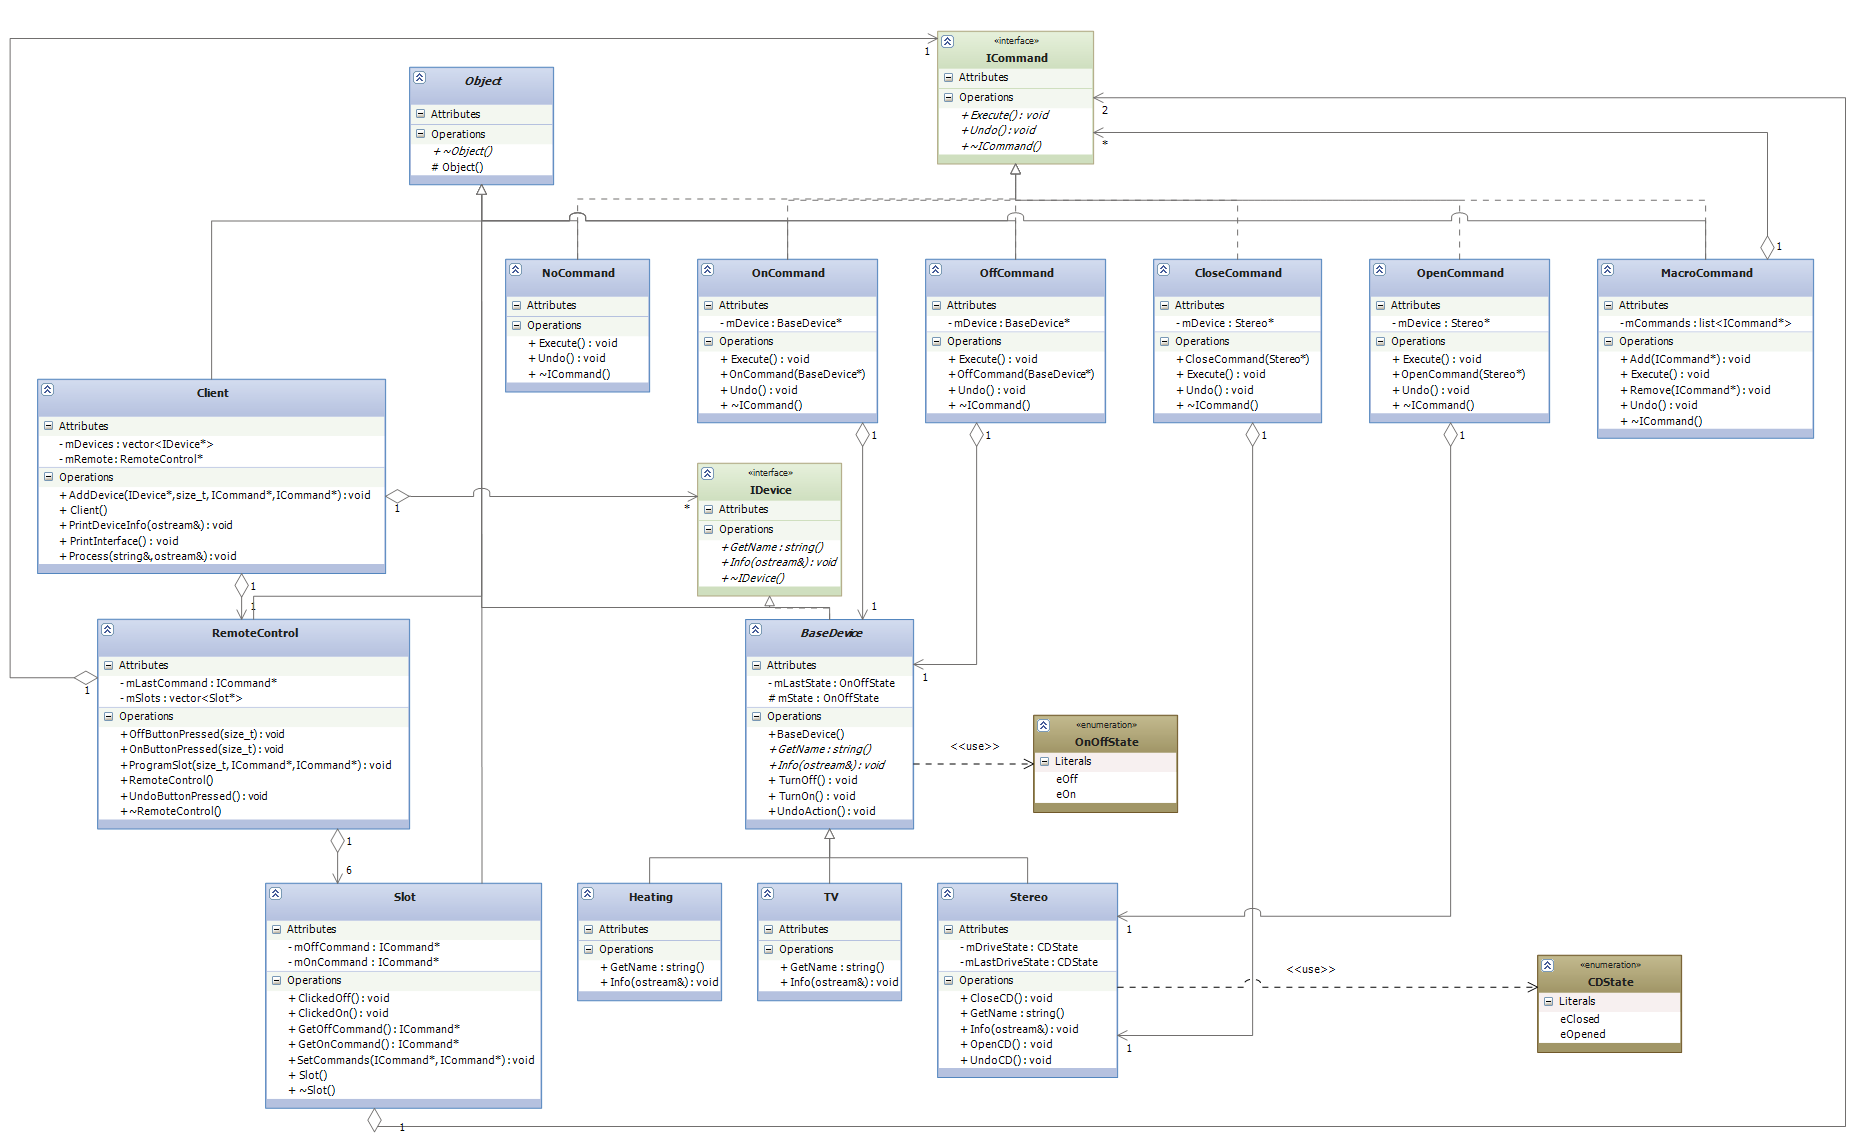
\includegraphics[angle=90,scale=0.55] {../Klassendiagramm.png}

\newpage
\subsection {Komponentenübersicht}
\begin {itemize} 
	\item Klasse "Object":
	\newline
	Basis aller Basisklassen.
	
	\item Klasse "Client":
	\newline
	Verwaltet die Geräte und kann deren Informationen ausgeben und verarbeitet die Eingaben vom Benutzer.

	\item Klasse "RemoteControl":
	\newline
	Verwaltet die Slots und kann die Slots programmieren.

	\item Klasse "Slot":
	\newline
	Verwaltet die Kommandos eines Slots.

	\item Interface "ICommand":
	\newline
	Schnittstellenbeschreibung für die Kommandos.
	
	\item Klassen "OffCommand, OnCommand, CloseCommand und OpenCommand":
	\newline
	Konkrete Kommandoklassen.

	\item Klasse "NoCommand":
	\newline
	Standard Kommando, das nur etwas ausgibt.
	
	\item Klasse "MacroCommand":
	\newline
	Zusammenfassung mehrerer Kommandos.

	\item Interface "IDevice":
	\newline
	Schnittstellenbeschreibung für die Geräte.
	
	\item Klasse "BaseDevice":
	\newline
	Basisklasse für die Geräte.

	\item Klassen "Heating, TV und Stereo":
	\newline
	Konkrete Geräteklassen.

	\item Enumeration "CDState":
	\newline
	Status des CD-Laufwerks.

	\item Enumeration "OnOffState":
	\newline
	Status ob ein- oder ausgeschalten.

			
\end {itemize}

\newpage
\section {Komponentenentwurf}
\subsection {Klasse "Object"}
Abstrakte Basisklasse aller Klassen. Von ihr werden alle anderen Klassen abgeleitet. Beinhaltet einen virtuellen Destruktor.

\subsection {Klasse "Client"}
Hat eine Liste die die Geräte verwaltet und einen Member der eine Referenz auf die Fernsteuerung speichert.
\\

\textbf {Methode "AddDevice": } 
\newline
Schnittstelle:
\newline
Parameter: IDevice*, size\_t
\newline
Rückgabetyp: void
\newline
Fügt der Liste ein Gerät hinzu. Falsche Eingaben werden berücksichtigt. Ruft ProgramSlot von der Fernbedienung auf.
\\

\textbf {Methode "PrintDeviceInfo": } 
\newline
Schnittstelle:
\newline
Parameter: ostream\&
\newline
Rückgabetyp: void
\newline
Gibt die Informationen der Geräte auf dem mitgegebenen Stream aus.
\\

\textbf {Methode "PrintInterface": } 
\newline
Schnittstelle:
\newline
Rückgabetyp: void
\newline
Gibt das Kommandozeilen-Interface auf der Konsole aus.
\\

\textbf {Methode "Process": } 
\newline
Schnittstelle:
\newline
Parameter: string\&
\newline
Rückgabetyp: void
\newline
Verarbeitet den in der Konsole eingegebenen string und ruft die dazugehörigen Methoden der Fernsteuerung auf.
\\

\subsection {Klasse "RemoteControl"}
Hat einen Vektor der Referenzen auf die Slots speichert und einen Member der das letzte Kommando speichert.
\\

\textbf {Konstruktor "RemoteControl": } 
\newline
Erstellt die Slots und setzt die Kommandos auf NoCommand.
\\

\textbf {Methode "OffButtonPressed": } 
\newline
Schnittstelle:
\newline
Parameter: size\_t
\newline
Rückgabetyp: void
\newline
Speichert das aktuelle Kommando im Member und ruft das Off-Kommando vom entsprechenden Slot auf.
\\

\textbf {Methode "OnButtonPressed": } 
\newline
Schnittstelle:
\newline
Parameter: size\_t
\newline
Rückgabetyp: void
\newline
Speichert das aktuelle Kommando im Member und ruft das On-Kommando vom entsprechenden Slot auf.
\\

\textbf {Methode "UndoButtonPressed": } 
\newline
Schnittstelle:
\newline
Rückgabetyp: void
\newline
Ruft vom letzten Kommando die Methode Undo auf und setzt den Pointer auf 0, weil nur ein Mal zurückgesetzt werden kann.
\\

\textbf {Methode "ProgramSlot": } 
\newline
Schnittstelle:
\newline
Parameter: size\_t, ICommand*, ICommand*
\newline
Rückgabetyp: void
\newline
Mit dieser Methode werden die Slots der Fernbedienung programmiert, das heißt die Kommandos werden zugewiesen.
\\

\subsection {Klasse "Slot"}
Speichert einen Pointer auf ein On- und ein Offkommando. Hat 2 Get-Methoden für diese und einen Destruktor der sie freigibt.
\\

\textbf {Konstruktor "Slot": } 
\newline
Weißt den Kommandozeigern 0 zu.
\\

\textbf {Methode "ClickedOff": } 
\newline
Schnittstelle:
\newline
Rückgabetyp: void
\newline
Überprüft den Pointer und ruft "Execute" vom Off-Kommando auf.
\\

\textbf {Methode "ClickedOn": } 
\newline
Schnittstelle:
\newline
Rückgabetyp: void
\newline
Überprüft den Pointer und ruft "Execute" vom On-Kommando auf.
\\

\textbf {Methode "SetCommands": } 
\newline
Schnittstelle:
\newline
Parameter: ICommand*, ICommand*
\newline
Rückgabetyp: void
\newline
Weist die Kommandos zu.
\\

\subsection {Interface "ICommand"}
Schnittstellendefiniton. Hat einen virtuellen Destruktor.
\\

\textbf {Methode "Execute": } 
\newline
Schnittstelle:
\newline
Rückgabetyp: void
\\

\textbf {Methode "Undo": } 
\newline
Schnittstelle:
\newline
Rückgabetyp: void
\\

\subsection {Klassen "OffCommand, OnCommand, CloseCommand, OpenCommand und NoCommand"}
Implementieren die Methoden Execute und Undo entsprechend der jeweiligen Klasse. Bei NoCommand wird einfach auf der Konsole ausgegeben, dass es sich um NoCommand handelt. Die anderen Kommandos rufen die entsprechenden Methoden in den Klassen, auf die sie eine Referenz haben, auf.
Sie haben weiters einen Konstruktor dem diese Referenzen mitgegeben werden.
\\

\subsection {Klasse "MacroCommand"}
Hat eine Liste die die Referenzen auf mehrere Kommandos speichert. Der Liste können die Kommandos hinzugefügt werden, aber auch wieder entfernt werden. Es können nur maximal 2 Elemente in der Liste gespeichert werden.
\\




\newpage
\section {Source Code}

%\lstinputlisting[language=C++]{\CodePath Object.h}
%\lstinputlisting[language=C++]{\CodePath Object.cpp}
%\newpage
%
%\lstinputlisting[language=C++]{\CodePath ICar.h}
%\newpage
%
%\lstinputlisting[language=C++]{\CodePath ConcreteCar.h}
%\newpage
%\lstinputlisting[language=C++]{\CodePath ConcreteCar.cpp}
%\newpage
%
%\lstinputlisting[language=C++]{\CodePath SmallCar.h}
%\newpage
%\lstinputlisting[language=C++]{\CodePath SmallCar.cpp}
%\newpage
%
%\lstinputlisting[language=C++]{\CodePath MiddleRangeCar.h}
%\newpage
%\lstinputlisting[language=C++]{\CodePath MiddleRangeCar.cpp}
%\newpage
%
%\lstinputlisting[language=C++]{\CodePath PremiumCar.h}
%\newpage
%\lstinputlisting[language=C++]{\CodePath PremiumCar.cpp}
%\newpage
%
%\lstinputlisting[language=C++]{\CodePath SUV.h}
%\newpage
%\lstinputlisting[language=C++]{\CodePath SUV.cpp}
%\newpage
%
%\lstinputlisting[language=C++]{\CodePath Decorator.h}
%\newpage
%\lstinputlisting[language=C++]{\CodePath Decorator.cpp}
%\newpage
%
%\lstinputlisting[language=C++]{\CodePath Decorator_AirConditioner.h}
%\newpage
%\lstinputlisting[language=C++]{\CodePath Decorator_AirConditioner.cpp}
%\newpage
%
%\lstinputlisting[language=C++]{\CodePath Decorator_Navi.h}
%\newpage
%\lstinputlisting[language=C++]{\CodePath Decorator_Navi.cpp}
%\newpage
%
%\lstinputlisting[language=C++]{\CodePath Decorator_Speedometer.h}
%\newpage
%\lstinputlisting[language=C++]{\CodePath Decorator_Speedometer.cpp}
%\newpage
%
%\lstinputlisting[language=C++]{\CodePath Decorator_Xenion.h}
%\newpage
%\lstinputlisting[language=C++]{\CodePath Decorator_Xenion.cpp}
%\newpage
%
%\lstinputlisting[language=C++]{\CodePath CarRental.h}
%\newpage
%\lstinputlisting[language=C++]{\CodePath CarRental.cpp}
%\newpage
%
%\lstinputlisting[language=C++]{\CodePath Main.cpp}
%\newpage

\section {Testausgaben} 

\begin {verbatim}
Visual Leak Detector Version 2.2.3 installed.
Empty testcase with NULL pointer.
Error in CarRental::Add: no valid pointer
Error in CarRental::MoveToAvailable: no valid pointer
Error in CarRental::Reserve: no valid pointer


Testcase with single entry
Add ...done
GetAvailable ...done
Reserve ...done
GetReserved ...done
PrintReserved ...Small Car: VW Golf - Price: 7500
Air Conditioner - Price: 1500
Total price: 9000
done
MoveToAvailable ...done
PrintAvailable ...Small Car: VW Golf - Price: 7500
Air Conditioner - Price: 1500
Total price: 9000
done


Testcase with several entries
Add ...done
GetAvailable ...done
Reserve ...done
GetReserved ...done
PrintReserved ...Premium Car: Audi R8 - Price: 45000
Xenion - Price: 3000
Navi - Price: 2000
Total price: 50000
SUV: Toyota RAV4 - Price: 22000
Total price: 22000
done
MoveToAvailable ...done
PrintAvailable ...Small Car: VW Golf - Price: 7500
Air Conditioner - Price: 1500
Total price: 9000
Middlerange Car: BMW 3 - Price: 16000
Speedometer - Price: 2500
Total price: 18500
SUV: Toyota RAV4 - Price: 22000
Total price: 22000
done


No memory leaks detected.
\end {verbatim}


\end{document}